\documentclass[11pt]{article}
\usepackage[textwidth=18.0cm, textheight=23.0cm, top=2.0cm]{geometry}
\usepackage{pst-all}
\usepackage{amssymb}
\usepackage{tikz}
\usepackage{underscore}\begin{document}
\pagestyle{empty}


ClassName: \underline{\textbf{Class_10.2bp-49}}
\par
BinSize: \underline{\textbf{100 × 100}}
\par
ReduceSize: \underline{\textbf{100 × 100}}
\par
TypeNum: \underline{\textbf{98}}
\par
Num: \underline{\textbf{100}}
\par
OutS: \underline{\textbf{150000}}
\par
InS: \underline{\textbf{141006}}
\par
Rate: \underline{\textbf{0.940}}
\par
UB: \underline{\textbf{15}}
\par
LB0: \underline{\textbf{15}}
\par
LB: \underline{\textbf{15}}
\par
LBWithCut: \underline{\textbf{15}}
\par
NodeCut: \underline{\textbf{0}}
\par
ExtendedNodeCnt: \underline{\textbf{1}}
\par
GenNodeCnt: \underline{\textbf{1}}
\par
PrimalNode: \underline{\textbf{0}}
\par
ColumnCount: \underline{\textbf{15}}
\par
TotalCutCount: \underline{\textbf{0}}
\par
RootCutCount: \underline{\textbf{0}}
\par
LPSolverCnt: \underline{\textbf{1}}
\par
PricingSolverCnt: \underline{\textbf{0}}
\par
BranchAndBoundNum: \underline{\textbf{1}}
\par
isOpt: \underline{\textbf{true}}
\par
TimeOnInitSolution: \underline{\textbf{600.000 s}}
\par
TimeOnPrimal: \underline{\textbf{0.000 s}}
\par
TimeOnPricing: \underline{\textbf{0.000 s}}
\par
TimeOnRmp: \underline{\textbf{0.078 s}}
\par
TotalTime: \underline{\textbf{600.328 s}}
\par
\newpage


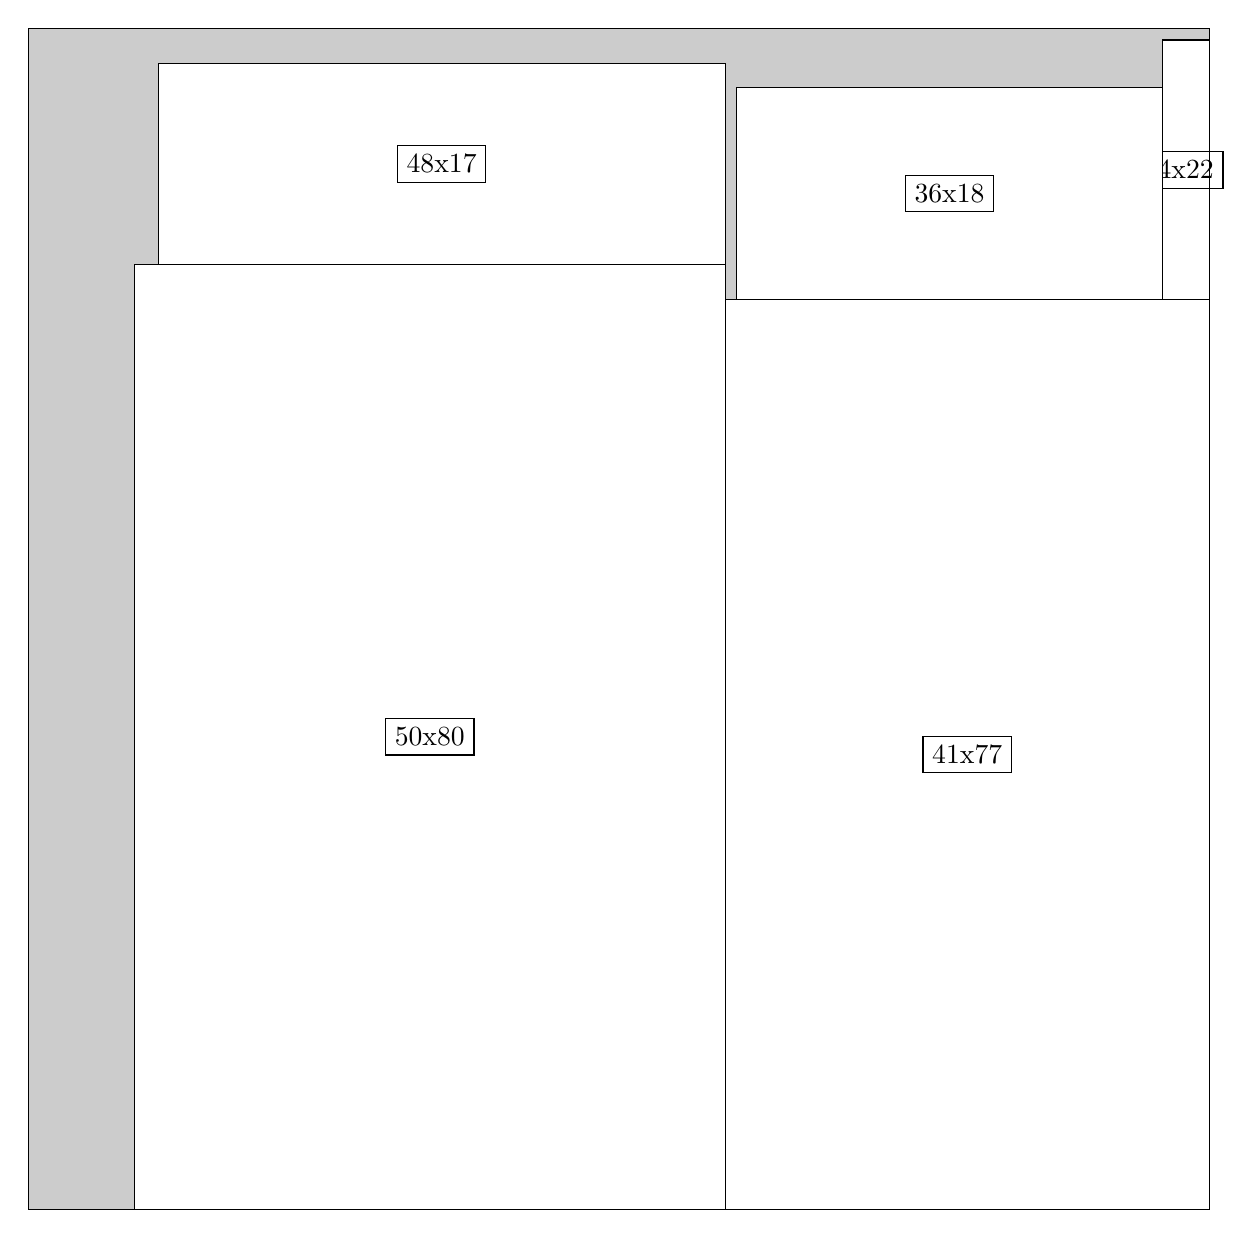
\begin{tikzpicture}[shorten >=1pt,scale=1.0,every node/.style={scale=1.0},->]
\tikzstyle{vertex}=[circle,fill=black!25,minimum size=14pt,inner sep=0pt]
\filldraw[fill=gray!40!white, draw=black] (0,0) rectangle (15.0,15.0);
\foreach \name/\x/\y/\w/\h in {41x77/8.85/0.0/6.1499999999999995/11.549999999999999,4x22/14.399999999999999/11.549999999999999/0.6/3.3,36x18/9.0/11.549999999999999/5.3999999999999995/2.6999999999999997,50x80/1.3499999999999999/0.0/7.5/12.0,48x17/1.65/12.0/7.199999999999999/2.55}
\filldraw[fill=white!40!white, draw=black] (\x,\y) rectangle node[draw] (\name) {\name} ++(\w,\h);
\end{tikzpicture}


w =41 , h =77 , x =59 , y =0 , v =3157
\par
w =4 , h =22 , x =96 , y =77 , v =88
\par
w =36 , h =18 , x =60 , y =77 , v =648
\par
w =50 , h =80 , x =9 , y =0 , v =4000
\par
w =48 , h =17 , x =11 , y =80 , v =816
\par
\newpage


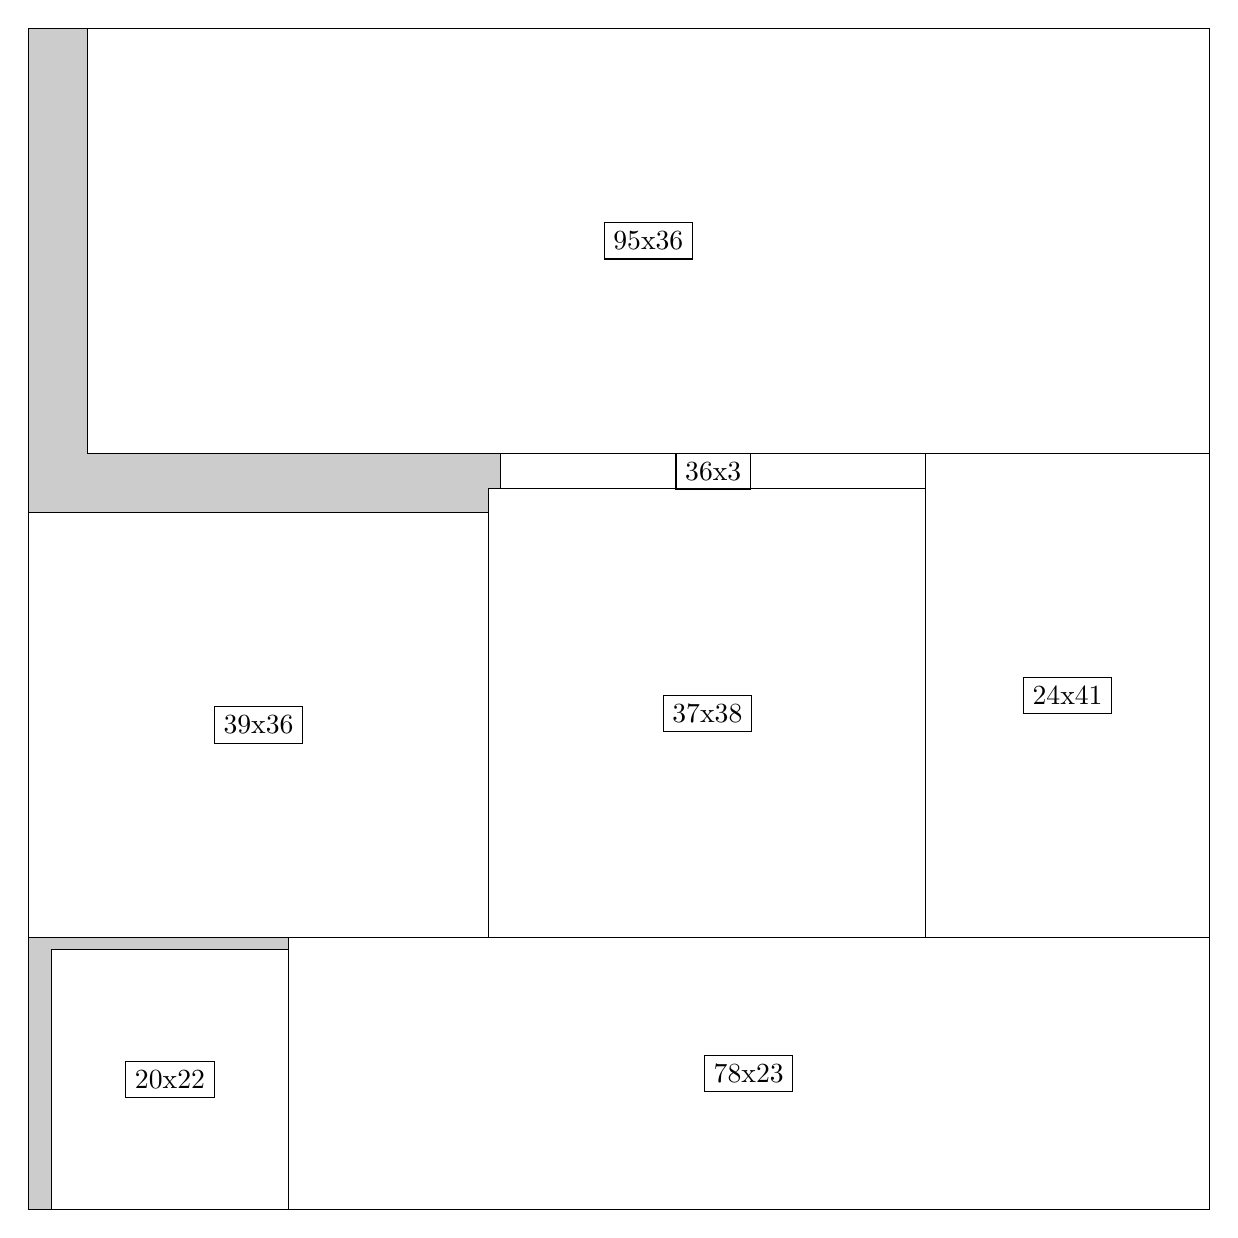
\begin{tikzpicture}[shorten >=1pt,scale=1.0,every node/.style={scale=1.0},->]
\tikzstyle{vertex}=[circle,fill=black!25,minimum size=14pt,inner sep=0pt]
\filldraw[fill=gray!40!white, draw=black] (0,0) rectangle (15.0,15.0);
\foreach \name/\x/\y/\w/\h in {78x23/3.3/0.0/11.7/3.4499999999999997,20x22/0.3/0.0/3.0/3.3,24x41/11.4/3.4499999999999997/3.5999999999999996/6.1499999999999995,37x38/5.85/3.4499999999999997/5.55/5.7,36x3/6.0/9.15/5.3999999999999995/0.44999999999999996,39x36/0.0/3.4499999999999997/5.85/5.3999999999999995,95x36/0.75/9.6/14.25/5.3999999999999995}
\filldraw[fill=white!40!white, draw=black] (\x,\y) rectangle node[draw] (\name) {\name} ++(\w,\h);
\end{tikzpicture}


w =78 , h =23 , x =22 , y =0 , v =1794
\par
w =20 , h =22 , x =2 , y =0 , v =440
\par
w =24 , h =41 , x =76 , y =23 , v =984
\par
w =37 , h =38 , x =39 , y =23 , v =1406
\par
w =36 , h =3 , x =40 , y =61 , v =108
\par
w =39 , h =36 , x =0 , y =23 , v =1404
\par
w =95 , h =36 , x =5 , y =64 , v =3420
\par
\newpage


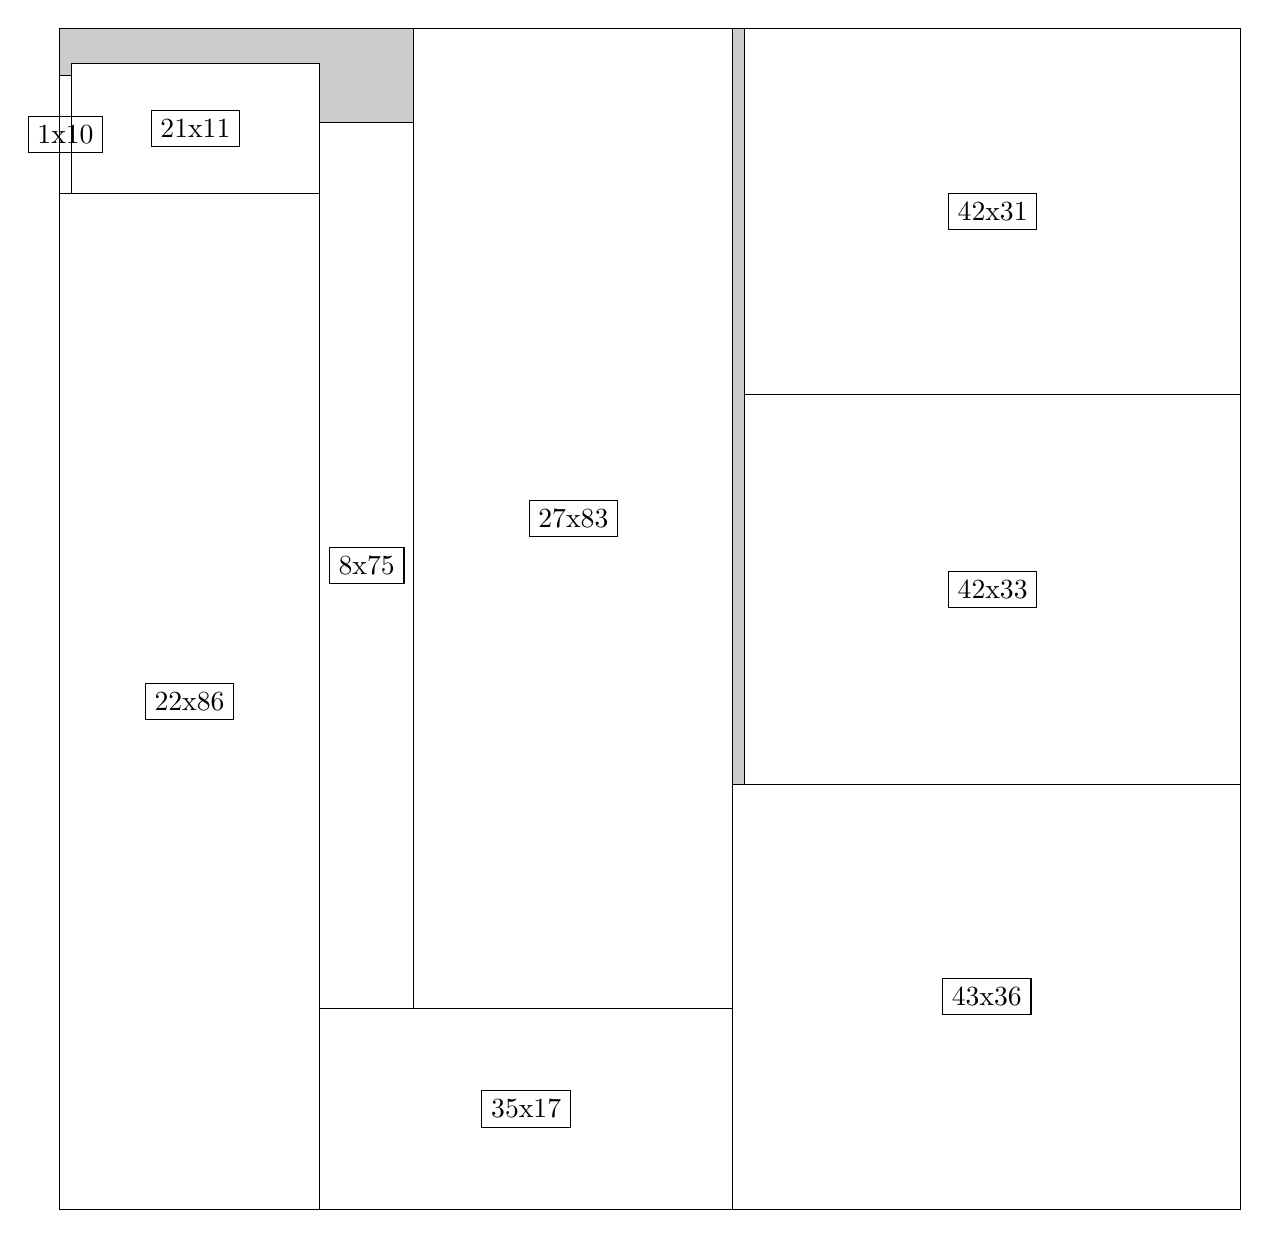
\begin{tikzpicture}[shorten >=1pt,scale=1.0,every node/.style={scale=1.0},->]
\tikzstyle{vertex}=[circle,fill=black!25,minimum size=14pt,inner sep=0pt]
\filldraw[fill=gray!40!white, draw=black] (0,0) rectangle (15.0,15.0);
\foreach \name/\x/\y/\w/\h in {43x36/8.549999999999999/0.0/6.45/5.3999999999999995,42x33/8.7/5.3999999999999995/6.3/4.95,42x31/8.7/10.35/6.3/4.6499999999999995,35x17/3.3/0.0/5.25/2.55,27x83/4.5/2.55/4.05/12.45,8x75/3.3/2.55/1.2/11.25,22x86/0.0/0.0/3.3/12.9,21x11/0.15/12.9/3.15/1.65,1x10/0.0/12.9/0.15/1.5}
\filldraw[fill=white!40!white, draw=black] (\x,\y) rectangle node[draw] (\name) {\name} ++(\w,\h);
\end{tikzpicture}


w =43 , h =36 , x =57 , y =0 , v =1548
\par
w =42 , h =33 , x =58 , y =36 , v =1386
\par
w =42 , h =31 , x =58 , y =69 , v =1302
\par
w =35 , h =17 , x =22 , y =0 , v =595
\par
w =27 , h =83 , x =30 , y =17 , v =2241
\par
w =8 , h =75 , x =22 , y =17 , v =600
\par
w =22 , h =86 , x =0 , y =0 , v =1892
\par
w =21 , h =11 , x =1 , y =86 , v =231
\par
w =1 , h =10 , x =0 , y =86 , v =10
\par
\newpage


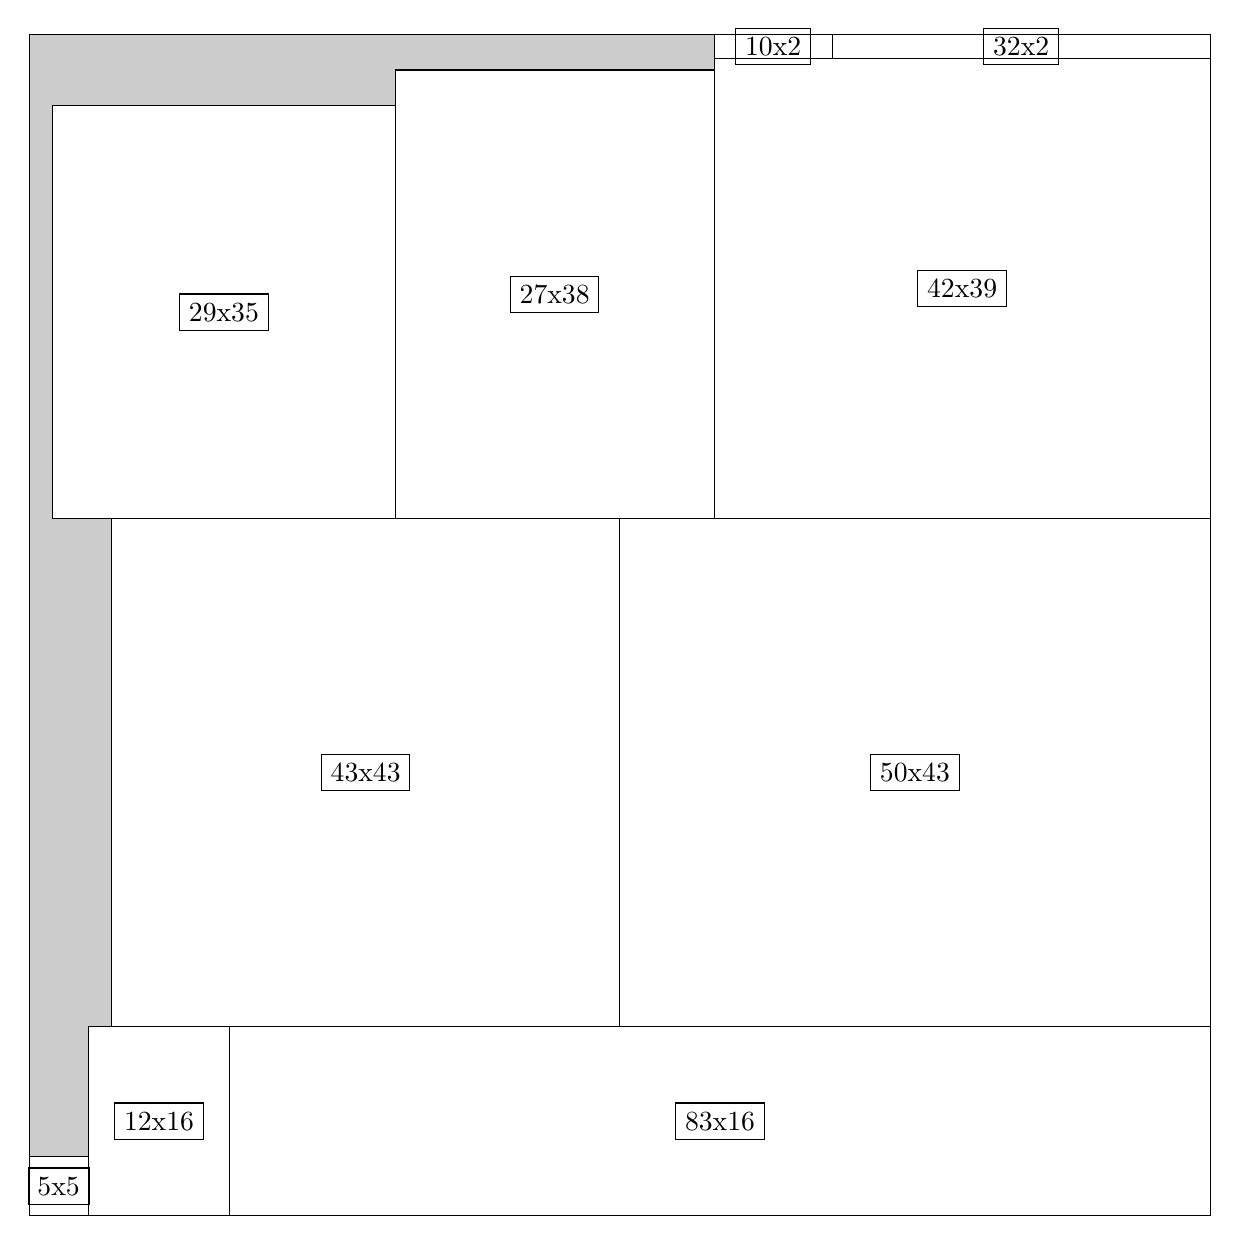
\begin{tikzpicture}[shorten >=1pt,scale=1.0,every node/.style={scale=1.0},->]
\tikzstyle{vertex}=[circle,fill=black!25,minimum size=14pt,inner sep=0pt]
\filldraw[fill=gray!40!white, draw=black] (0,0) rectangle (15.0,15.0);
\foreach \name/\x/\y/\w/\h in {83x16/2.55/0.0/12.45/2.4,12x16/0.75/0.0/1.7999999999999998/2.4,5x5/0.0/0.0/0.75/0.75,50x43/7.5/2.4/7.5/6.45,43x43/1.05/2.4/6.45/6.45,42x39/8.7/8.85/6.3/5.85,32x2/10.2/14.7/4.8/0.3,10x2/8.7/14.7/1.5/0.3,27x38/4.6499999999999995/8.85/4.05/5.7,29x35/0.3/8.85/4.35/5.25}
\filldraw[fill=white!40!white, draw=black] (\x,\y) rectangle node[draw] (\name) {\name} ++(\w,\h);
\end{tikzpicture}


w =83 , h =16 , x =17 , y =0 , v =1328
\par
w =12 , h =16 , x =5 , y =0 , v =192
\par
w =5 , h =5 , x =0 , y =0 , v =25
\par
w =50 , h =43 , x =50 , y =16 , v =2150
\par
w =43 , h =43 , x =7 , y =16 , v =1849
\par
w =42 , h =39 , x =58 , y =59 , v =1638
\par
w =32 , h =2 , x =68 , y =98 , v =64
\par
w =10 , h =2 , x =58 , y =98 , v =20
\par
w =27 , h =38 , x =31 , y =59 , v =1026
\par
w =29 , h =35 , x =2 , y =59 , v =1015
\par
\newpage


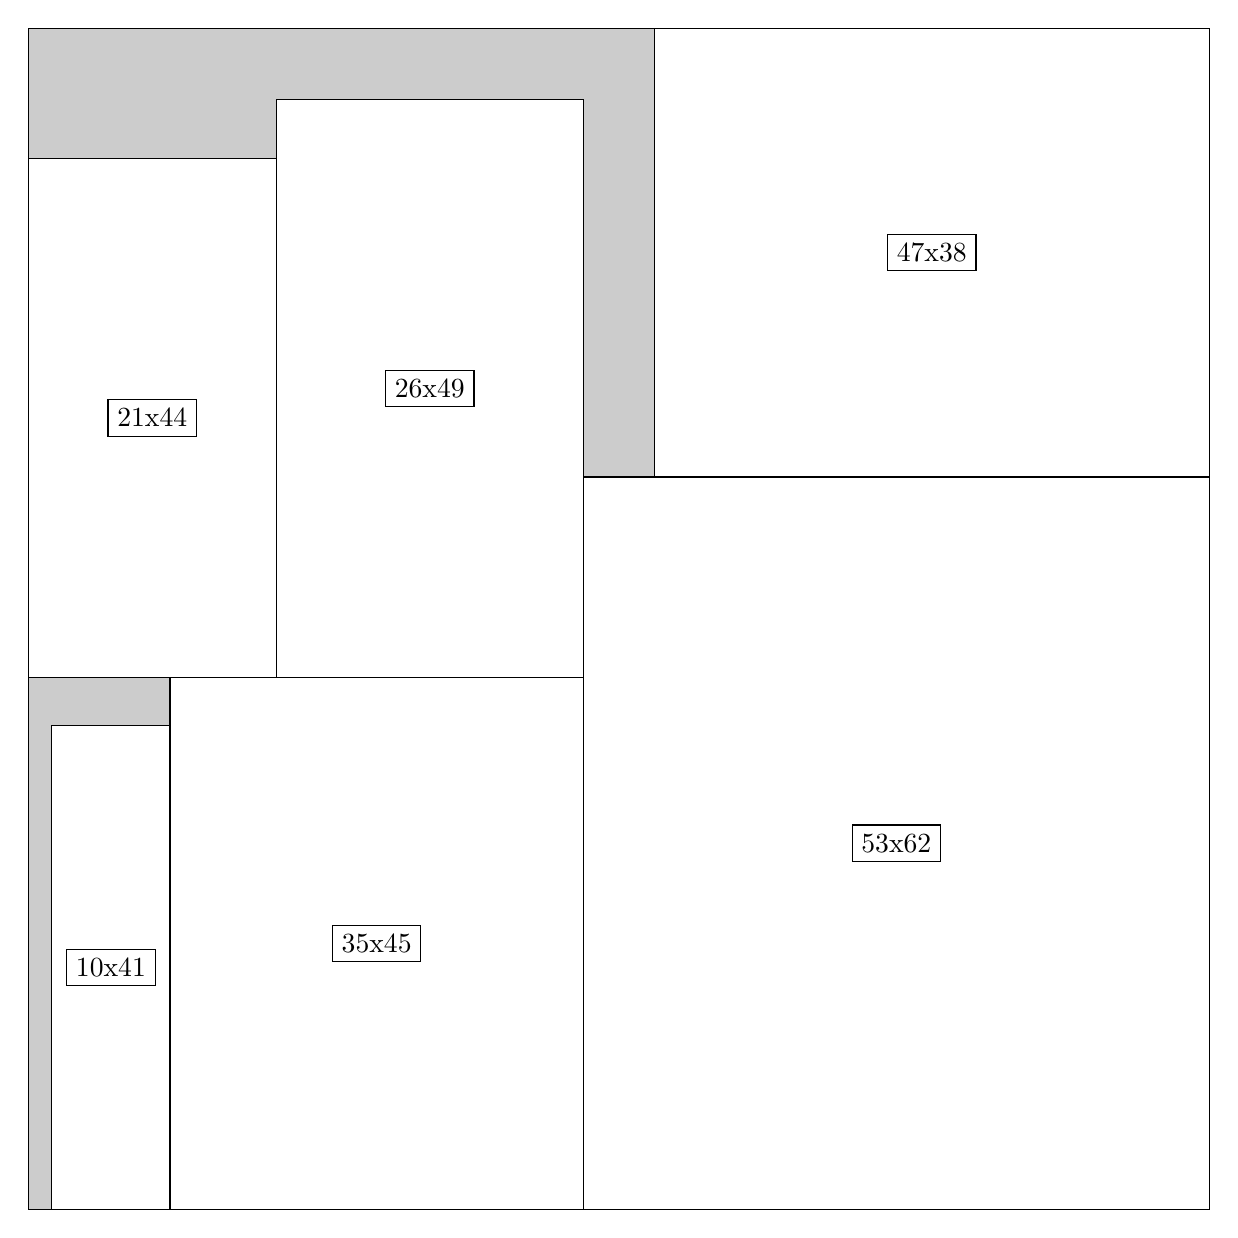
\begin{tikzpicture}[shorten >=1pt,scale=1.0,every node/.style={scale=1.0},->]
\tikzstyle{vertex}=[circle,fill=black!25,minimum size=14pt,inner sep=0pt]
\filldraw[fill=gray!40!white, draw=black] (0,0) rectangle (15.0,15.0);
\foreach \name/\x/\y/\w/\h in {53x62/7.05/0.0/7.949999999999999/9.299999999999999,47x38/7.949999999999999/9.299999999999999/7.05/5.7,35x45/1.7999999999999998/0.0/5.25/6.75,10x41/0.3/0.0/1.5/6.1499999999999995,26x49/3.15/6.75/3.9/7.35,21x44/0.0/6.75/3.15/6.6}
\filldraw[fill=white!40!white, draw=black] (\x,\y) rectangle node[draw] (\name) {\name} ++(\w,\h);
\end{tikzpicture}


w =53 , h =62 , x =47 , y =0 , v =3286
\par
w =47 , h =38 , x =53 , y =62 , v =1786
\par
w =35 , h =45 , x =12 , y =0 , v =1575
\par
w =10 , h =41 , x =2 , y =0 , v =410
\par
w =26 , h =49 , x =21 , y =45 , v =1274
\par
w =21 , h =44 , x =0 , y =45 , v =924
\par
\newpage


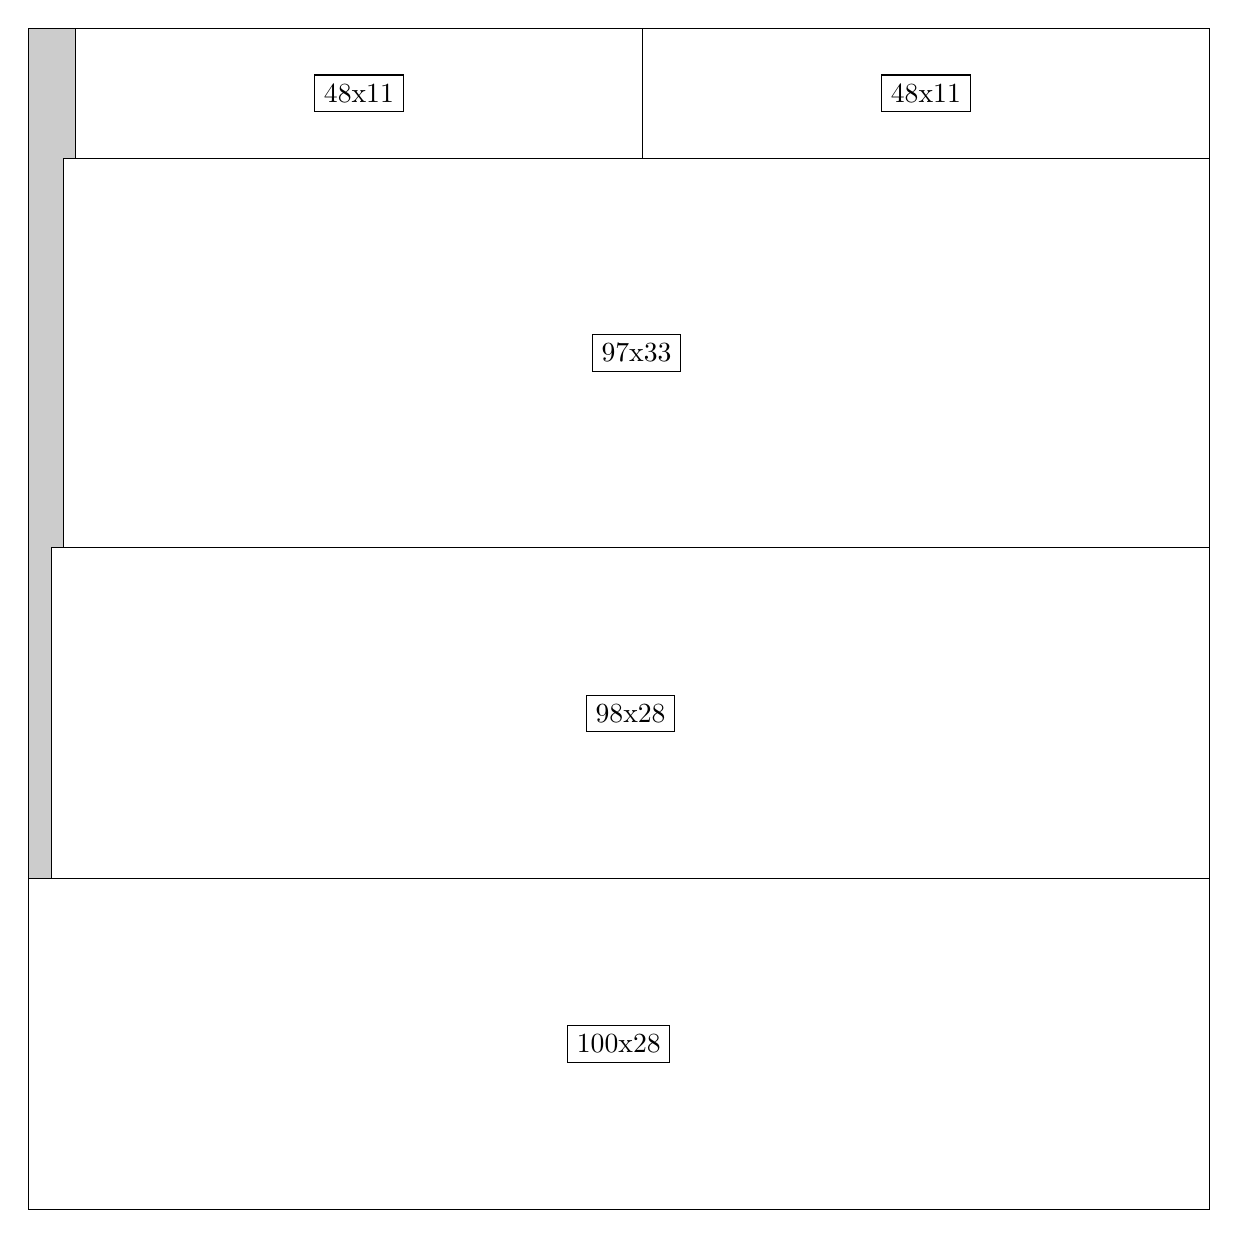
\begin{tikzpicture}[shorten >=1pt,scale=1.0,every node/.style={scale=1.0},->]
\tikzstyle{vertex}=[circle,fill=black!25,minimum size=14pt,inner sep=0pt]
\filldraw[fill=gray!40!white, draw=black] (0,0) rectangle (15.0,15.0);
\foreach \name/\x/\y/\w/\h in {100x28/0.0/0.0/15.0/4.2,98x28/0.3/4.2/14.7/4.2,97x33/0.44999999999999996/8.4/14.549999999999999/4.95,48x11/7.8/13.35/7.199999999999999/1.65,48x11/0.6/13.35/7.199999999999999/1.65}
\filldraw[fill=white!40!white, draw=black] (\x,\y) rectangle node[draw] (\name) {\name} ++(\w,\h);
\end{tikzpicture}


w =100 , h =28 , x =0 , y =0 , v =2800
\par
w =98 , h =28 , x =2 , y =28 , v =2744
\par
w =97 , h =33 , x =3 , y =56 , v =3201
\par
w =48 , h =11 , x =52 , y =89 , v =528
\par
w =48 , h =11 , x =4 , y =89 , v =528
\par
\newpage


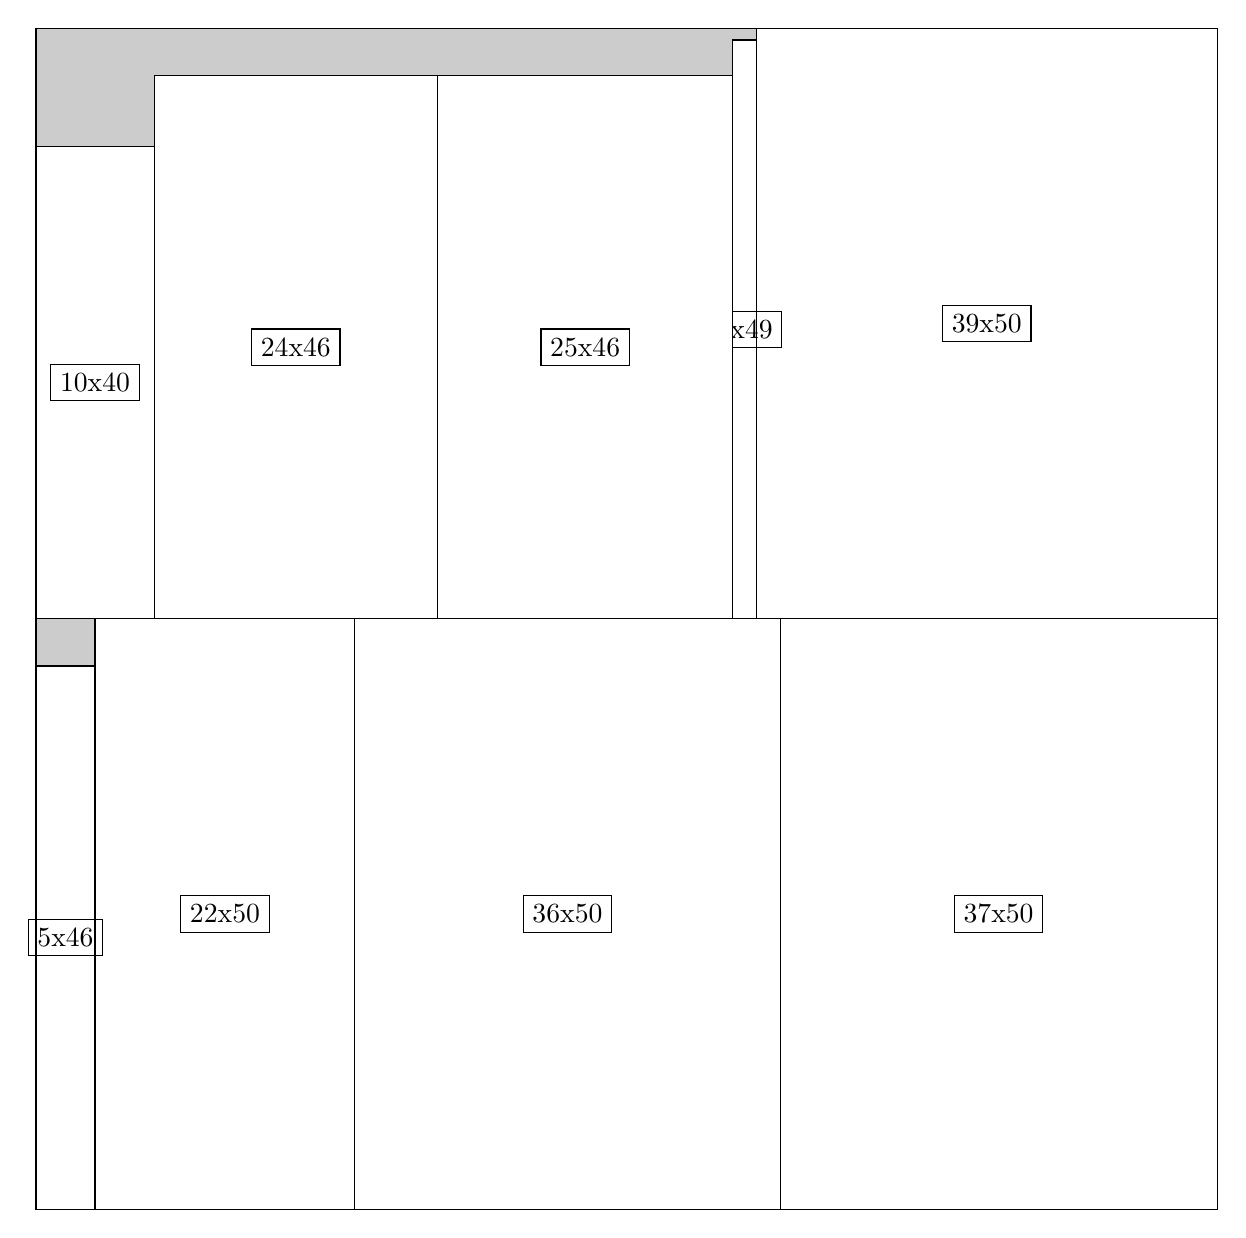
\begin{tikzpicture}[shorten >=1pt,scale=1.0,every node/.style={scale=1.0},->]
\tikzstyle{vertex}=[circle,fill=black!25,minimum size=14pt,inner sep=0pt]
\filldraw[fill=gray!40!white, draw=black] (0,0) rectangle (15.0,15.0);
\foreach \name/\x/\y/\w/\h in {37x50/9.45/0.0/5.55/7.5,36x50/4.05/0.0/5.3999999999999995/7.5,22x50/0.75/0.0/3.3/7.5,5x46/0.0/0.0/0.75/6.8999999999999995,39x50/9.15/7.5/5.85/7.5,2x49/8.85/7.5/0.3/7.35,25x46/5.1/7.5/3.75/6.8999999999999995,24x46/1.5/7.5/3.5999999999999996/6.8999999999999995,10x40/0.0/7.5/1.5/6.0}
\filldraw[fill=white!40!white, draw=black] (\x,\y) rectangle node[draw] (\name) {\name} ++(\w,\h);
\end{tikzpicture}


w =37 , h =50 , x =63 , y =0 , v =1850
\par
w =36 , h =50 , x =27 , y =0 , v =1800
\par
w =22 , h =50 , x =5 , y =0 , v =1100
\par
w =5 , h =46 , x =0 , y =0 , v =230
\par
w =39 , h =50 , x =61 , y =50 , v =1950
\par
w =2 , h =49 , x =59 , y =50 , v =98
\par
w =25 , h =46 , x =34 , y =50 , v =1150
\par
w =24 , h =46 , x =10 , y =50 , v =1104
\par
w =10 , h =40 , x =0 , y =50 , v =400
\par
\newpage


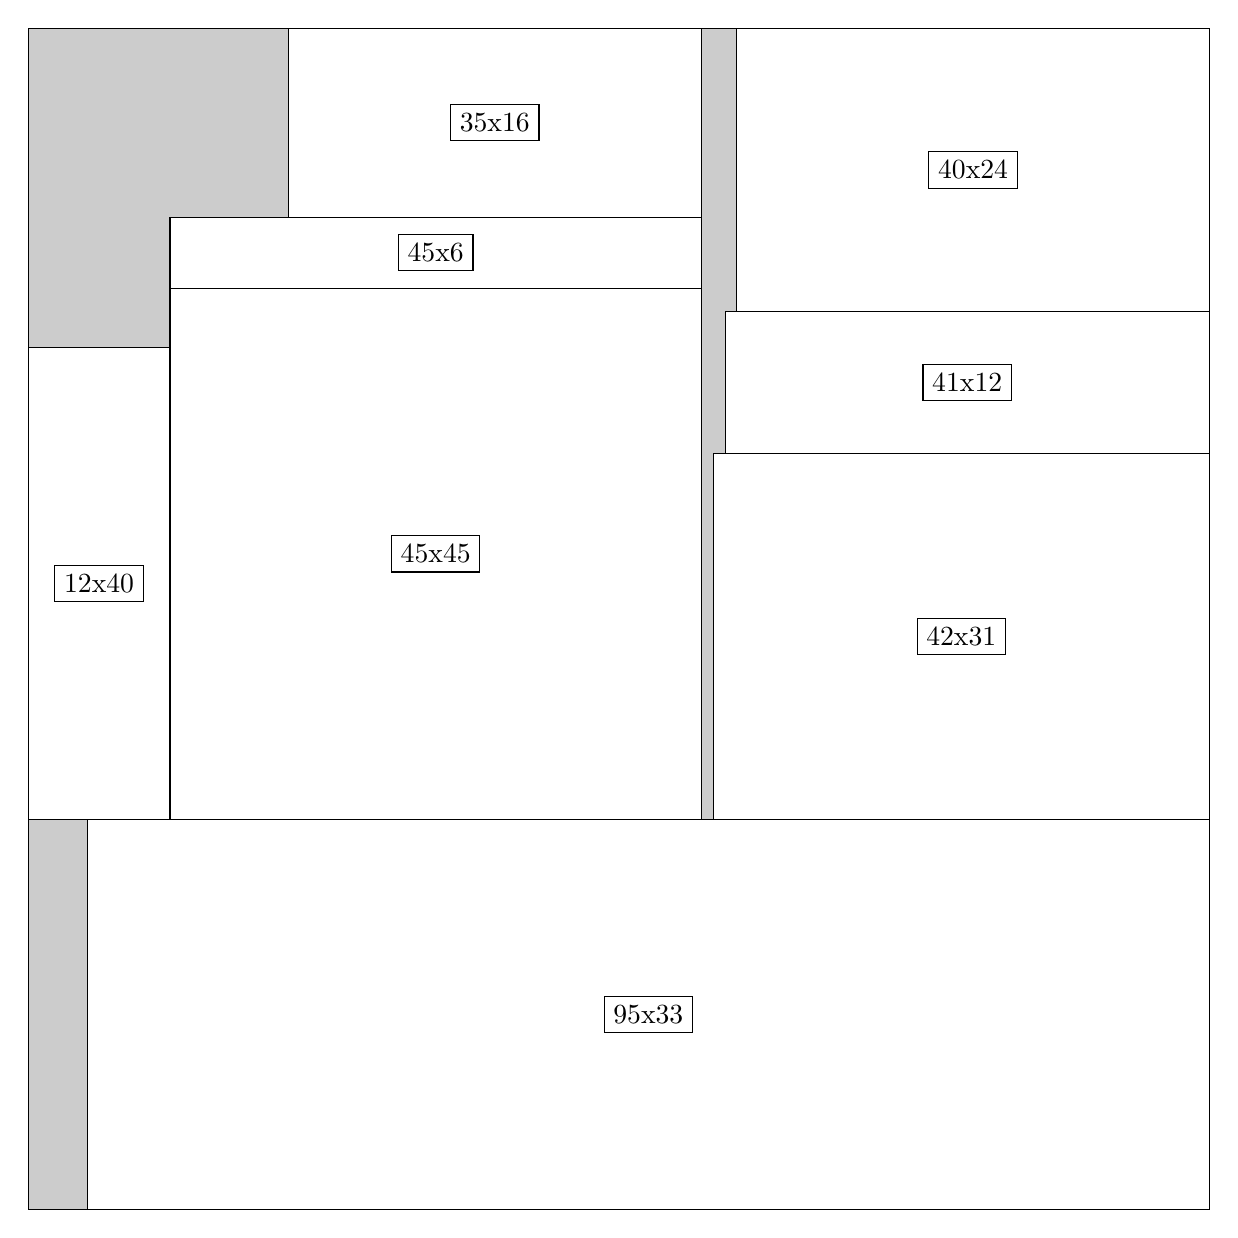
\begin{tikzpicture}[shorten >=1pt,scale=1.0,every node/.style={scale=1.0},->]
\tikzstyle{vertex}=[circle,fill=black!25,minimum size=14pt,inner sep=0pt]
\filldraw[fill=gray!40!white, draw=black] (0,0) rectangle (15.0,15.0);
\foreach \name/\x/\y/\w/\h in {95x33/0.75/0.0/14.25/4.95,42x31/8.7/4.95/6.3/4.6499999999999995,41x12/8.85/9.6/6.1499999999999995/1.7999999999999998,40x24/9.0/11.4/6.0/3.5999999999999996,45x45/1.7999999999999998/4.95/6.75/6.75,45x6/1.7999999999999998/11.7/6.75/0.8999999999999999,35x16/3.3/12.6/5.25/2.4,12x40/0.0/4.95/1.7999999999999998/6.0}
\filldraw[fill=white!40!white, draw=black] (\x,\y) rectangle node[draw] (\name) {\name} ++(\w,\h);
\end{tikzpicture}


w =95 , h =33 , x =5 , y =0 , v =3135
\par
w =42 , h =31 , x =58 , y =33 , v =1302
\par
w =41 , h =12 , x =59 , y =64 , v =492
\par
w =40 , h =24 , x =60 , y =76 , v =960
\par
w =45 , h =45 , x =12 , y =33 , v =2025
\par
w =45 , h =6 , x =12 , y =78 , v =270
\par
w =35 , h =16 , x =22 , y =84 , v =560
\par
w =12 , h =40 , x =0 , y =33 , v =480
\par
\newpage


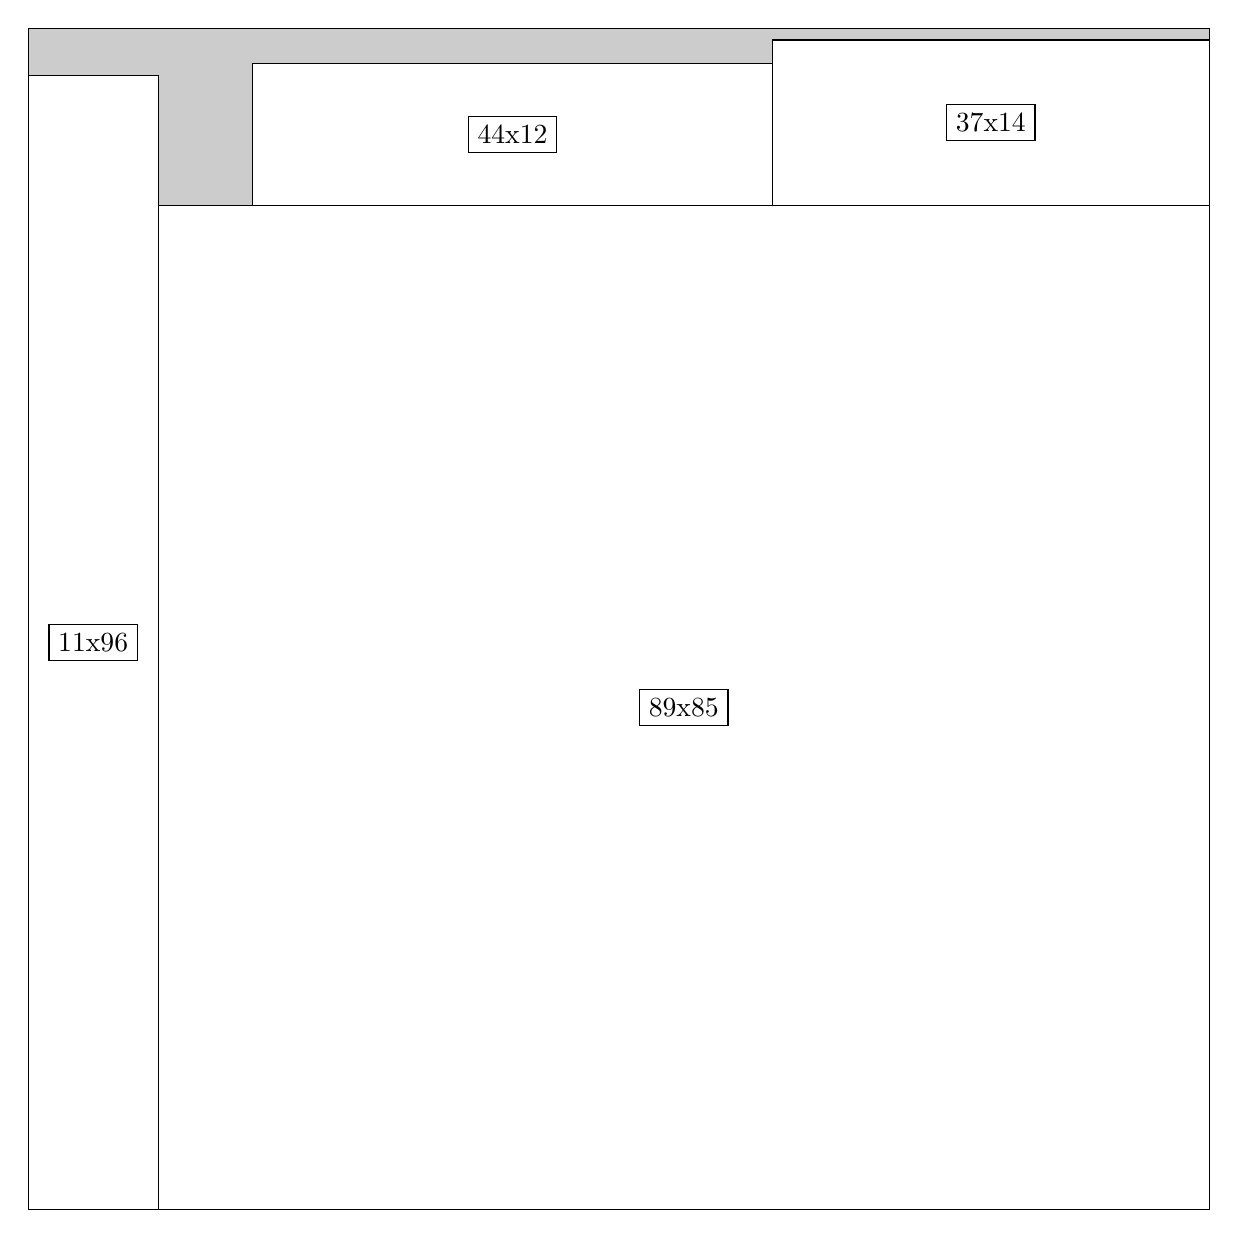
\begin{tikzpicture}[shorten >=1pt,scale=1.0,every node/.style={scale=1.0},->]
\tikzstyle{vertex}=[circle,fill=black!25,minimum size=14pt,inner sep=0pt]
\filldraw[fill=gray!40!white, draw=black] (0,0) rectangle (15.0,15.0);
\foreach \name/\x/\y/\w/\h in {89x85/1.65/0.0/13.35/12.75,37x14/9.45/12.75/5.55/2.1,44x12/2.85/12.75/6.6/1.7999999999999998,11x96/0.0/0.0/1.65/14.399999999999999}
\filldraw[fill=white!40!white, draw=black] (\x,\y) rectangle node[draw] (\name) {\name} ++(\w,\h);
\end{tikzpicture}


w =89 , h =85 , x =11 , y =0 , v =7565
\par
w =37 , h =14 , x =63 , y =85 , v =518
\par
w =44 , h =12 , x =19 , y =85 , v =528
\par
w =11 , h =96 , x =0 , y =0 , v =1056
\par
\newpage


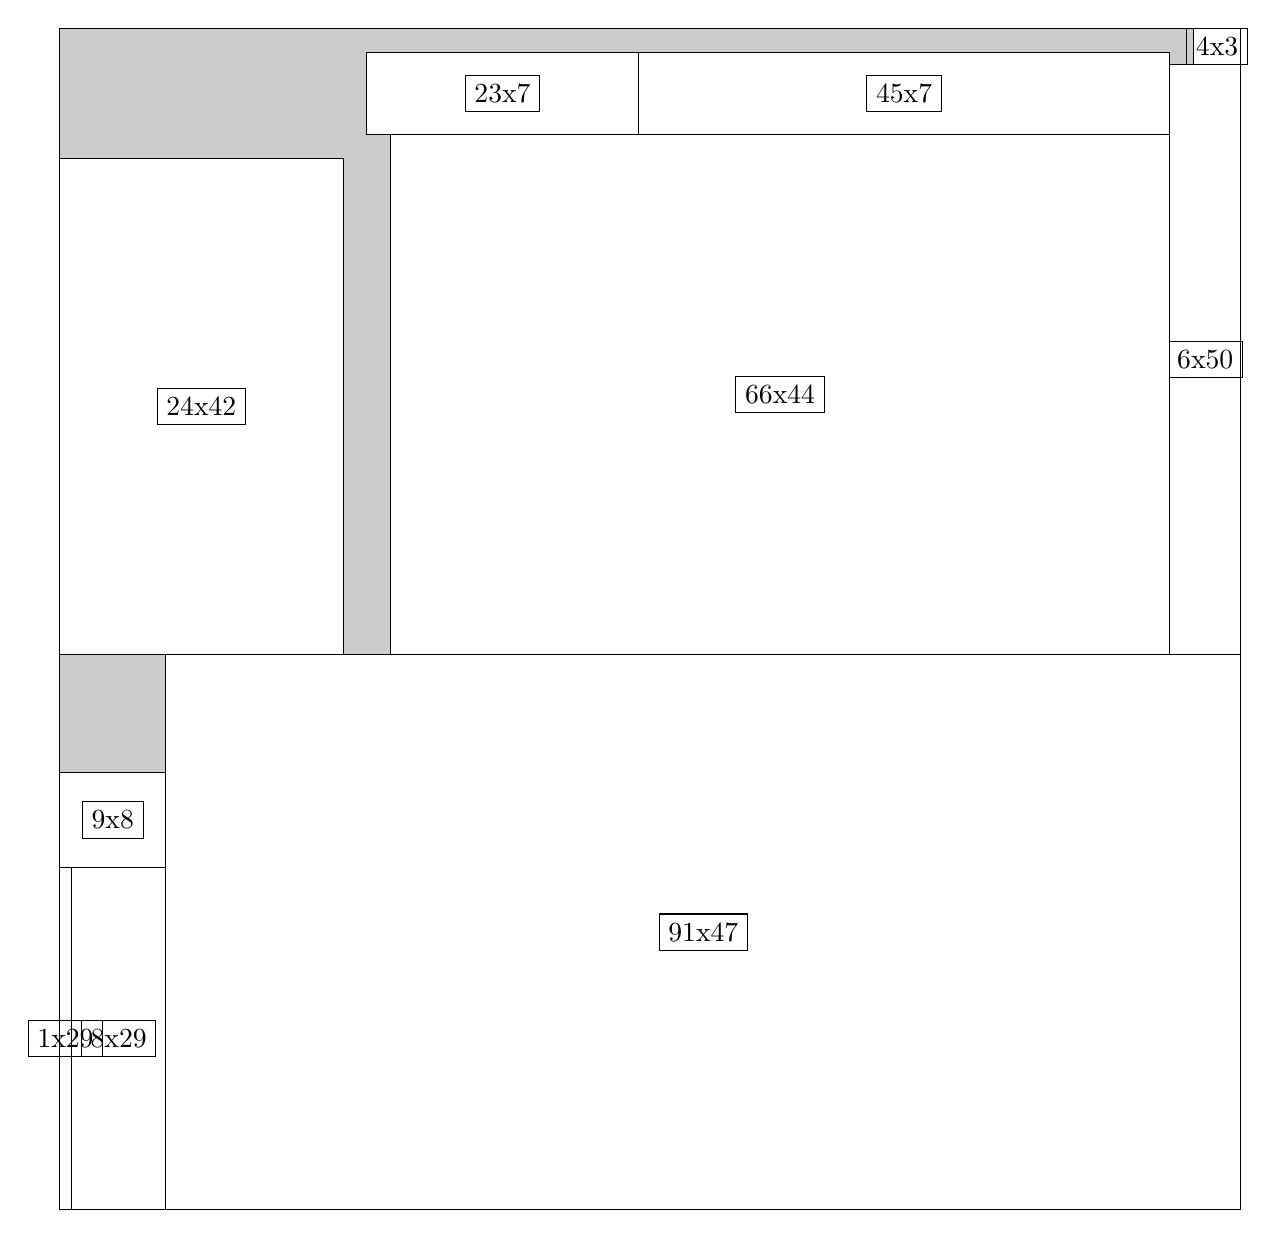
\begin{tikzpicture}[shorten >=1pt,scale=1.0,every node/.style={scale=1.0},->]
\tikzstyle{vertex}=[circle,fill=black!25,minimum size=14pt,inner sep=0pt]
\filldraw[fill=gray!40!white, draw=black] (0,0) rectangle (15.0,15.0);
\foreach \name/\x/\y/\w/\h in {91x47/1.3499999999999999/0.0/13.65/7.05,8x29/0.15/0.0/1.2/4.35,1x29/0.0/0.0/0.15/4.35,9x8/0.0/4.35/1.3499999999999999/1.2,6x50/14.1/7.05/0.8999999999999999/7.5,4x3/14.399999999999999/14.549999999999999/0.6/0.44999999999999996,66x44/4.2/7.05/9.9/6.6,45x7/7.35/13.65/6.75/1.05,23x7/3.9/13.65/3.4499999999999997/1.05,24x42/0.0/7.05/3.5999999999999996/6.3}
\filldraw[fill=white!40!white, draw=black] (\x,\y) rectangle node[draw] (\name) {\name} ++(\w,\h);
\end{tikzpicture}


w =91 , h =47 , x =9 , y =0 , v =4277
\par
w =8 , h =29 , x =1 , y =0 , v =232
\par
w =1 , h =29 , x =0 , y =0 , v =29
\par
w =9 , h =8 , x =0 , y =29 , v =72
\par
w =6 , h =50 , x =94 , y =47 , v =300
\par
w =4 , h =3 , x =96 , y =97 , v =12
\par
w =66 , h =44 , x =28 , y =47 , v =2904
\par
w =45 , h =7 , x =49 , y =91 , v =315
\par
w =23 , h =7 , x =26 , y =91 , v =161
\par
w =24 , h =42 , x =0 , y =47 , v =1008
\par
\newpage


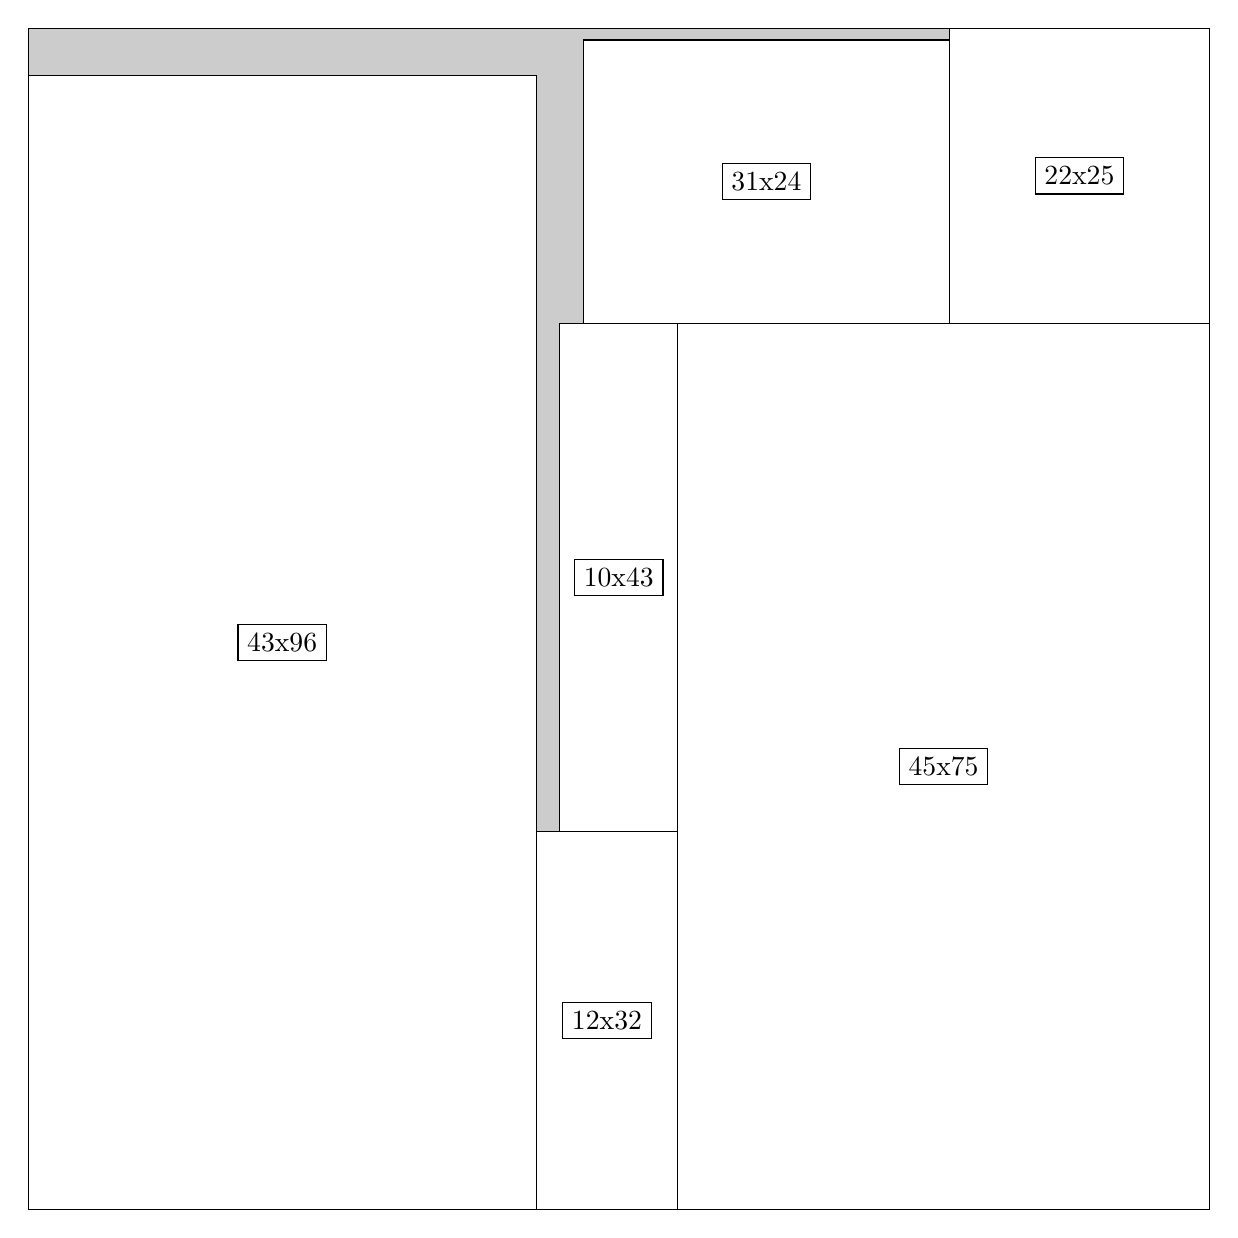
\begin{tikzpicture}[shorten >=1pt,scale=1.0,every node/.style={scale=1.0},->]
\tikzstyle{vertex}=[circle,fill=black!25,minimum size=14pt,inner sep=0pt]
\filldraw[fill=gray!40!white, draw=black] (0,0) rectangle (15.0,15.0);
\foreach \name/\x/\y/\w/\h in {45x75/8.25/0.0/6.75/11.25,12x32/6.45/0.0/1.7999999999999998/4.8,10x43/6.75/4.8/1.5/6.45,22x25/11.7/11.25/3.3/3.75,31x24/7.05/11.25/4.6499999999999995/3.5999999999999996,43x96/0.0/0.0/6.45/14.399999999999999}
\filldraw[fill=white!40!white, draw=black] (\x,\y) rectangle node[draw] (\name) {\name} ++(\w,\h);
\end{tikzpicture}


w =45 , h =75 , x =55 , y =0 , v =3375
\par
w =12 , h =32 , x =43 , y =0 , v =384
\par
w =10 , h =43 , x =45 , y =32 , v =430
\par
w =22 , h =25 , x =78 , y =75 , v =550
\par
w =31 , h =24 , x =47 , y =75 , v =744
\par
w =43 , h =96 , x =0 , y =0 , v =4128
\par
\newpage


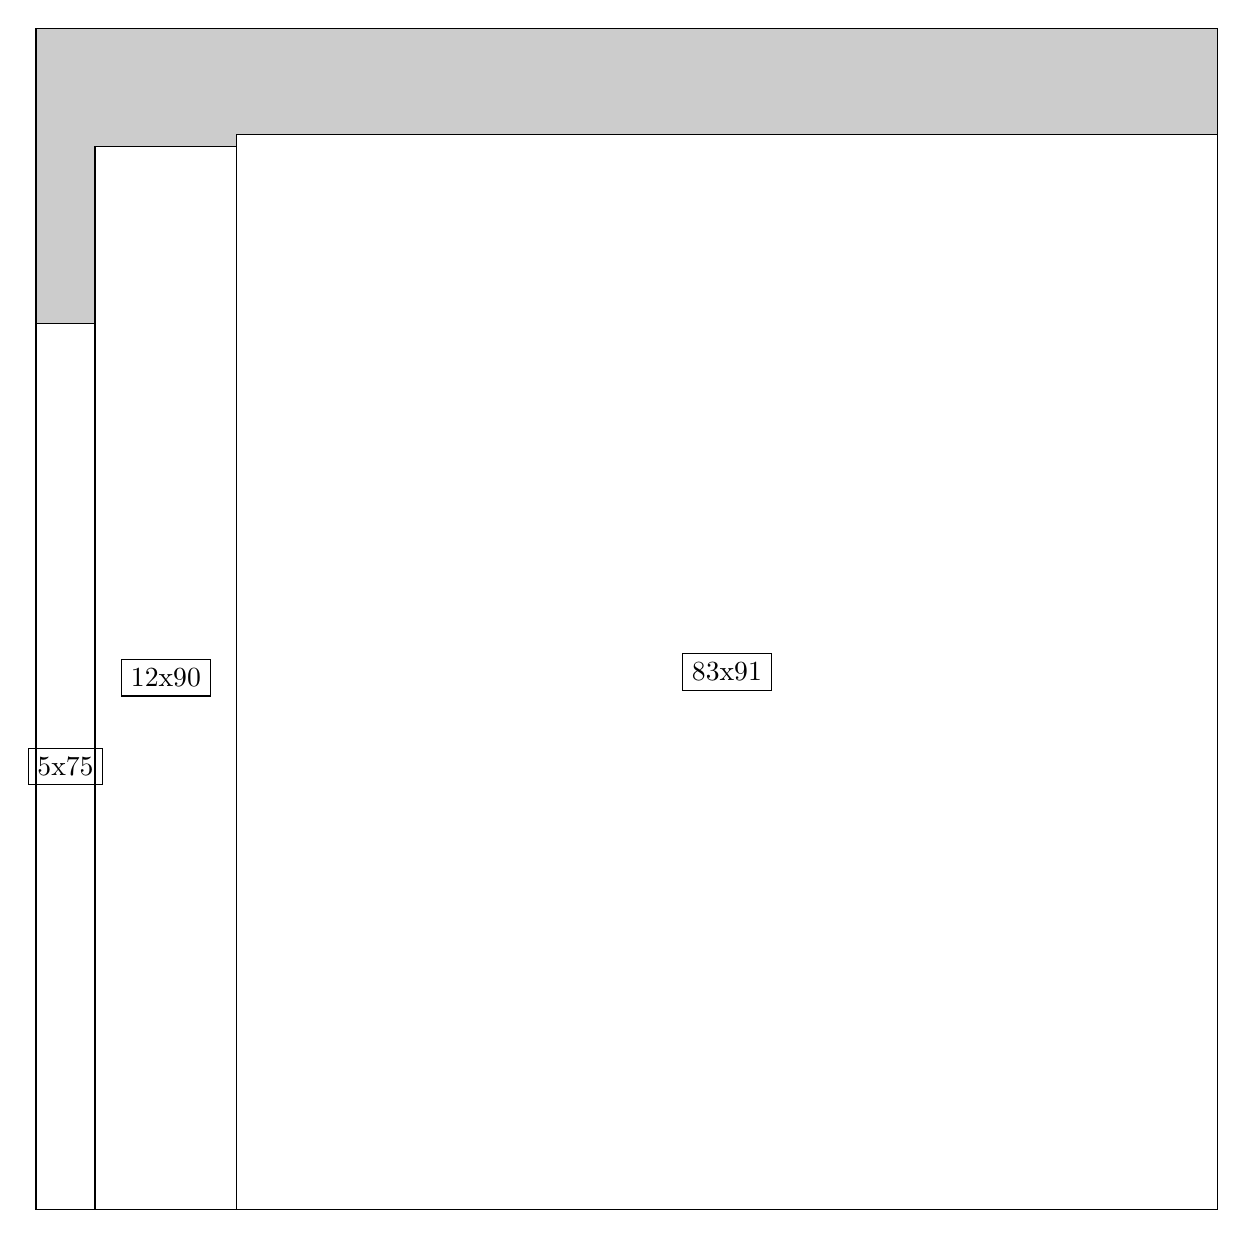
\begin{tikzpicture}[shorten >=1pt,scale=1.0,every node/.style={scale=1.0},->]
\tikzstyle{vertex}=[circle,fill=black!25,minimum size=14pt,inner sep=0pt]
\filldraw[fill=gray!40!white, draw=black] (0,0) rectangle (15.0,15.0);
\foreach \name/\x/\y/\w/\h in {83x91/2.55/0.0/12.45/13.65,12x90/0.75/0.0/1.7999999999999998/13.5,5x75/0.0/0.0/0.75/11.25}
\filldraw[fill=white!40!white, draw=black] (\x,\y) rectangle node[draw] (\name) {\name} ++(\w,\h);
\end{tikzpicture}


w =83 , h =91 , x =17 , y =0 , v =7553
\par
w =12 , h =90 , x =5 , y =0 , v =1080
\par
w =5 , h =75 , x =0 , y =0 , v =375
\par
\newpage


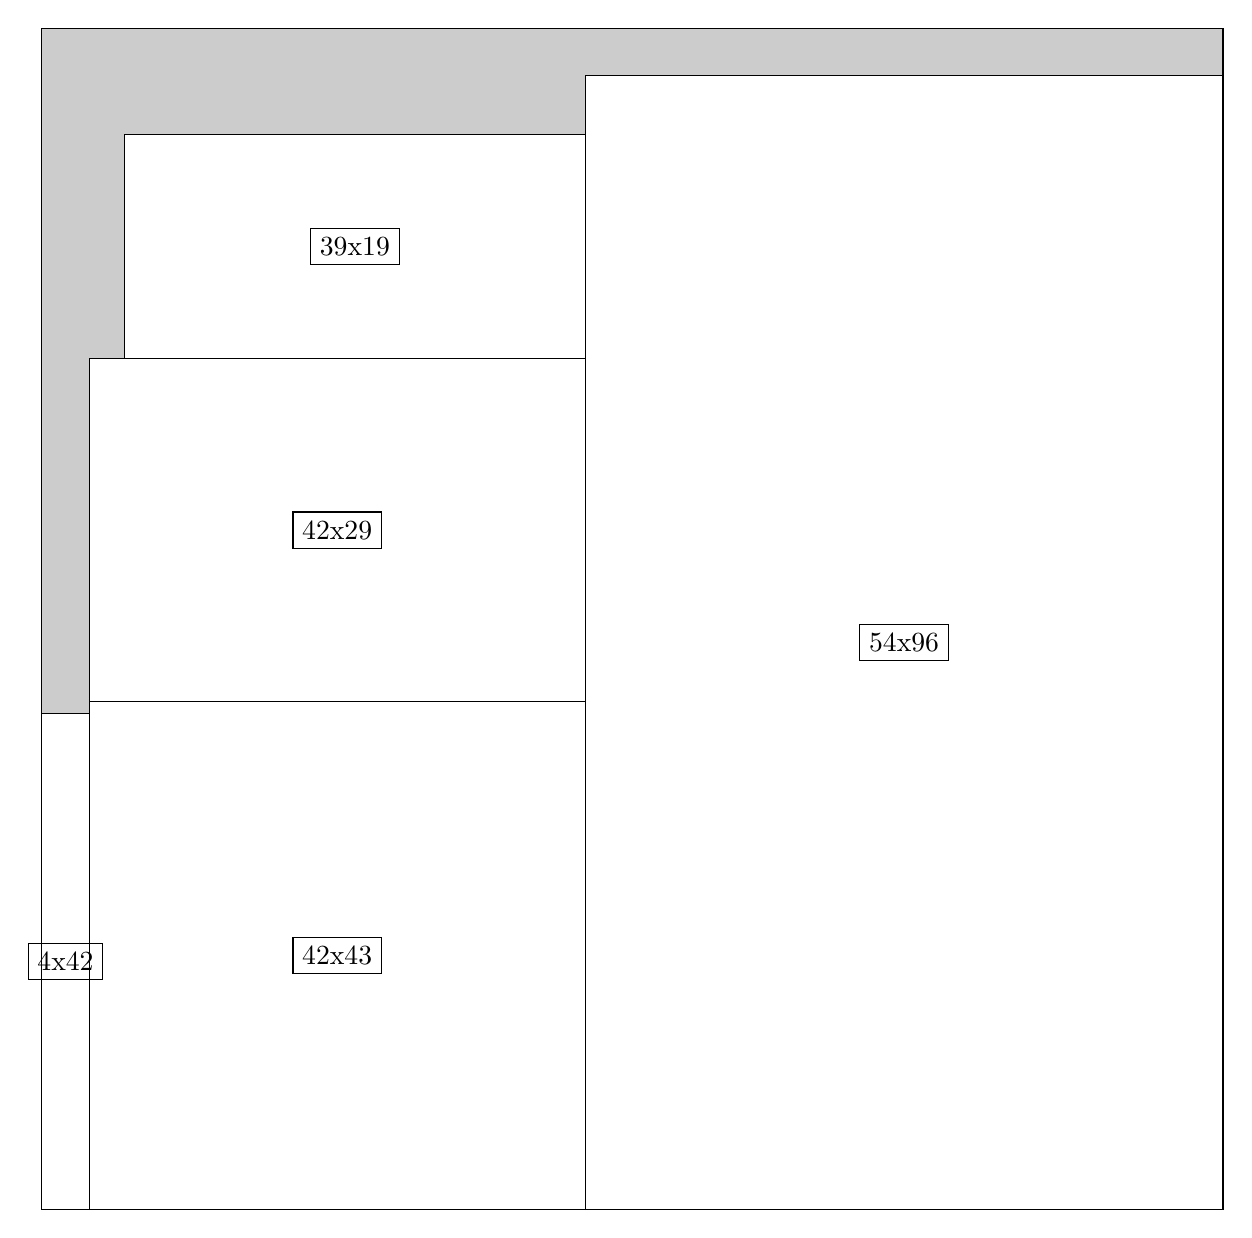
\begin{tikzpicture}[shorten >=1pt,scale=1.0,every node/.style={scale=1.0},->]
\tikzstyle{vertex}=[circle,fill=black!25,minimum size=14pt,inner sep=0pt]
\filldraw[fill=gray!40!white, draw=black] (0,0) rectangle (15.0,15.0);
\foreach \name/\x/\y/\w/\h in {54x96/6.8999999999999995/0.0/8.1/14.399999999999999,42x43/0.6/0.0/6.3/6.45,4x42/0.0/0.0/0.6/6.3,42x29/0.6/6.45/6.3/4.35,39x19/1.05/10.799999999999999/5.85/2.85}
\filldraw[fill=white!40!white, draw=black] (\x,\y) rectangle node[draw] (\name) {\name} ++(\w,\h);
\end{tikzpicture}


w =54 , h =96 , x =46 , y =0 , v =5184
\par
w =42 , h =43 , x =4 , y =0 , v =1806
\par
w =4 , h =42 , x =0 , y =0 , v =168
\par
w =42 , h =29 , x =4 , y =43 , v =1218
\par
w =39 , h =19 , x =7 , y =72 , v =741
\par
\newpage


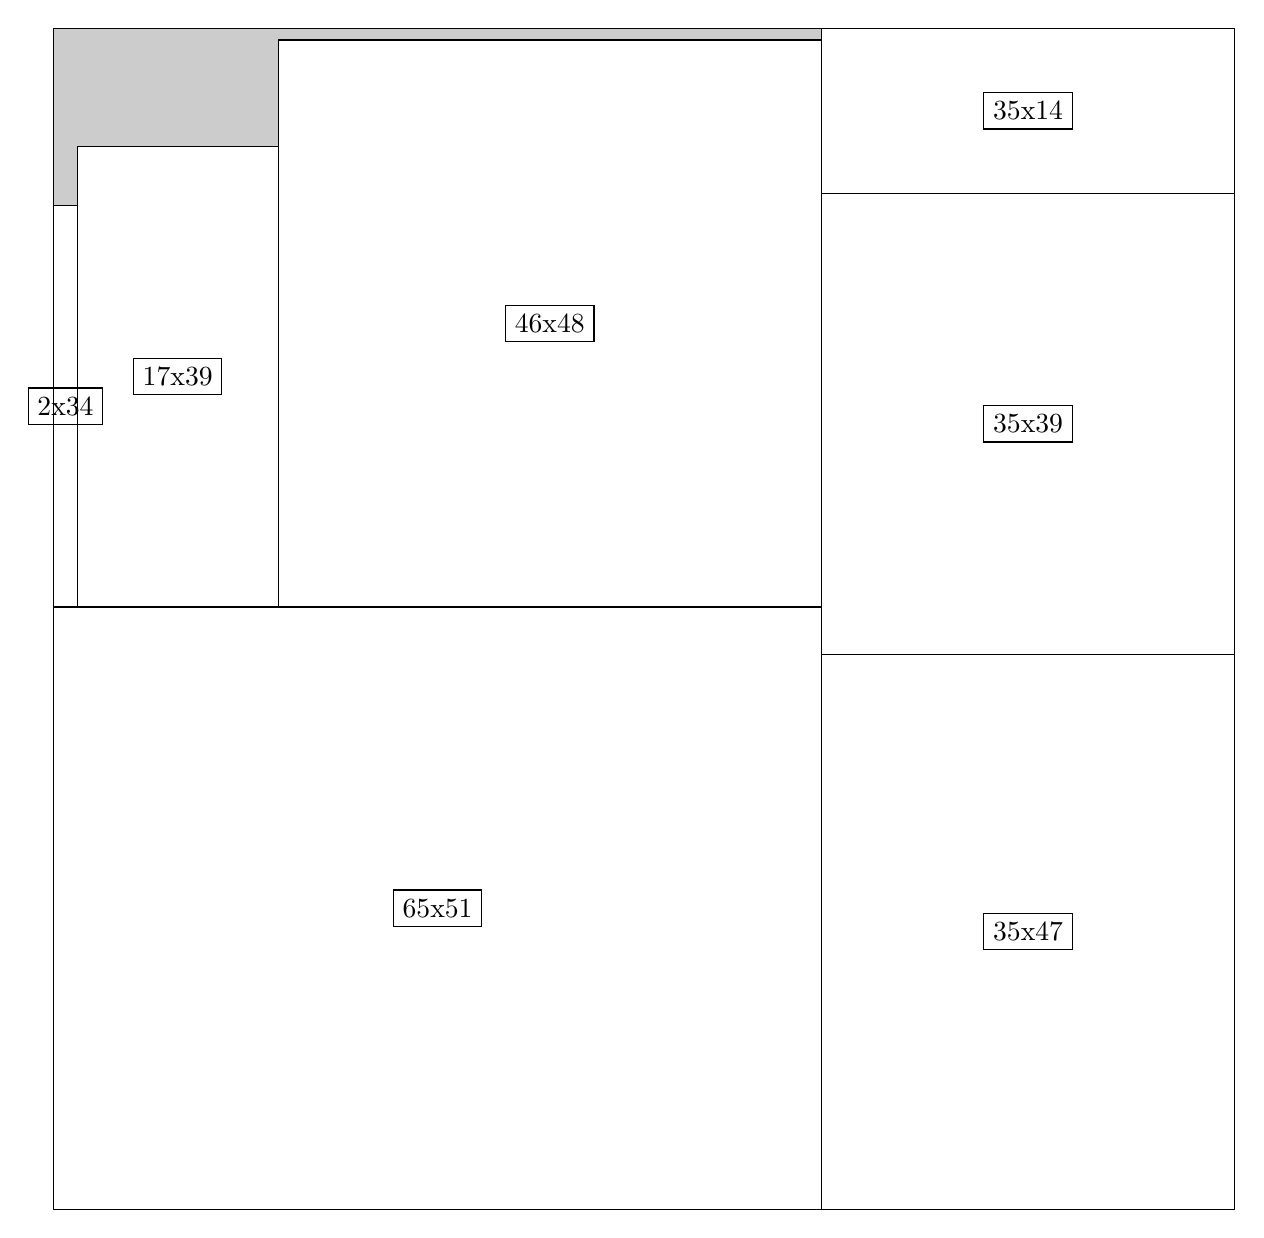
\begin{tikzpicture}[shorten >=1pt,scale=1.0,every node/.style={scale=1.0},->]
\tikzstyle{vertex}=[circle,fill=black!25,minimum size=14pt,inner sep=0pt]
\filldraw[fill=gray!40!white, draw=black] (0,0) rectangle (15.0,15.0);
\foreach \name/\x/\y/\w/\h in {35x47/9.75/0.0/5.25/7.05,35x39/9.75/7.05/5.25/5.85,35x14/9.75/12.9/5.25/2.1,65x51/0.0/0.0/9.75/7.6499999999999995,46x48/2.85/7.6499999999999995/6.8999999999999995/7.199999999999999,17x39/0.3/7.6499999999999995/2.55/5.85,2x34/0.0/7.6499999999999995/0.3/5.1}
\filldraw[fill=white!40!white, draw=black] (\x,\y) rectangle node[draw] (\name) {\name} ++(\w,\h);
\end{tikzpicture}


w =35 , h =47 , x =65 , y =0 , v =1645
\par
w =35 , h =39 , x =65 , y =47 , v =1365
\par
w =35 , h =14 , x =65 , y =86 , v =490
\par
w =65 , h =51 , x =0 , y =0 , v =3315
\par
w =46 , h =48 , x =19 , y =51 , v =2208
\par
w =17 , h =39 , x =2 , y =51 , v =663
\par
w =2 , h =34 , x =0 , y =51 , v =68
\par
\newpage


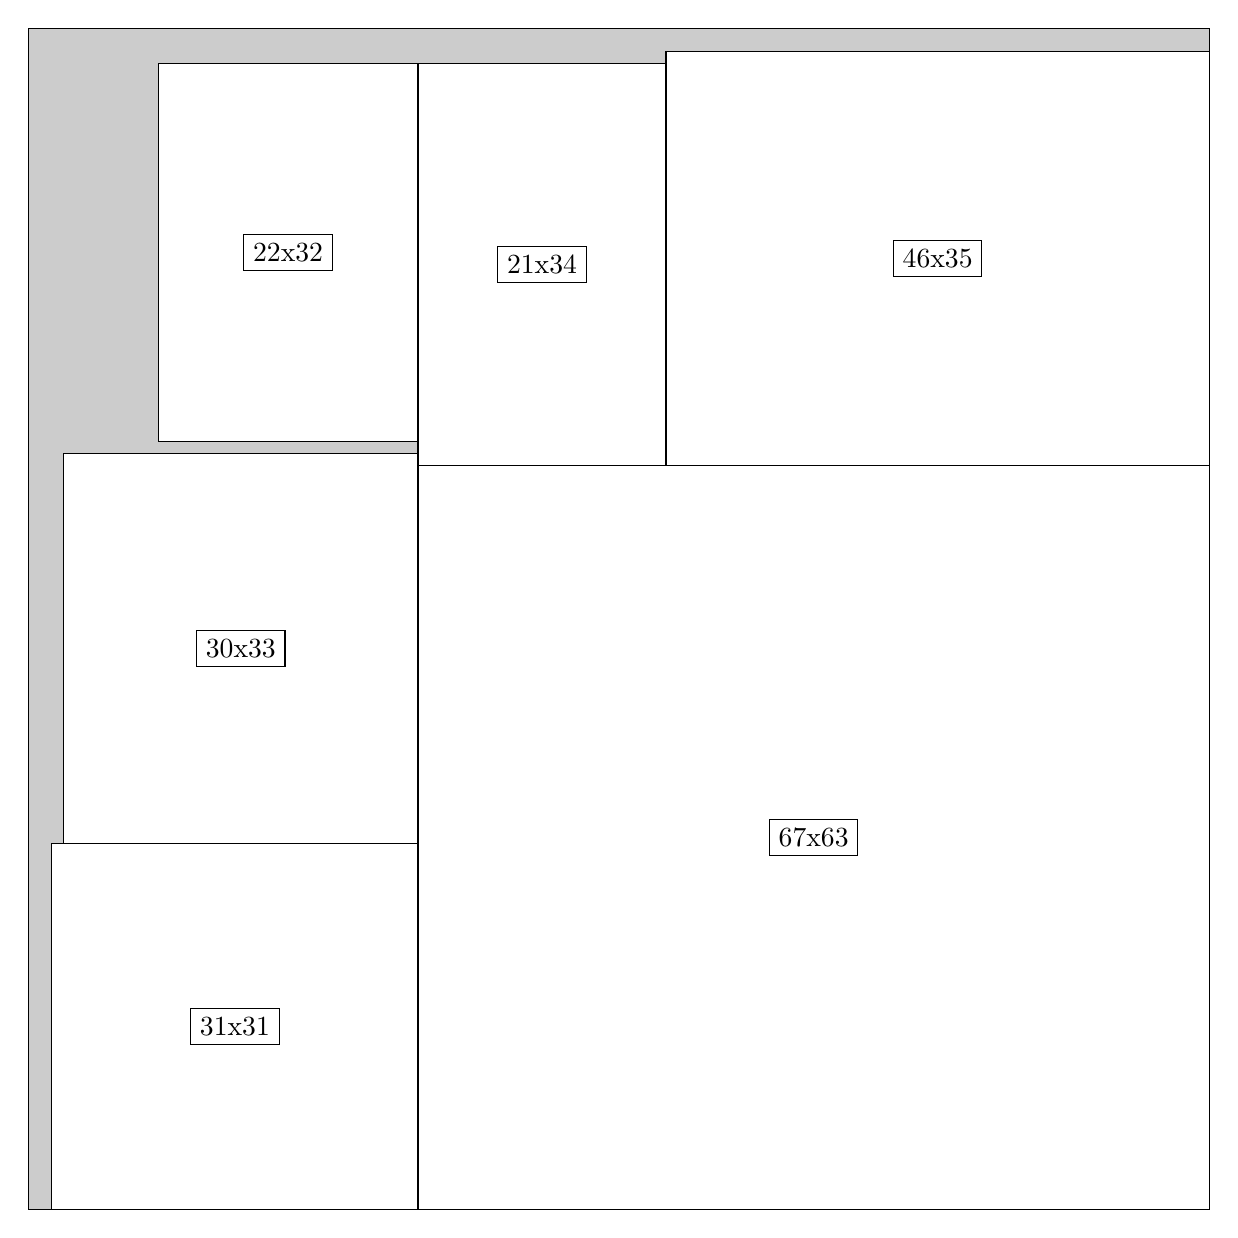
\begin{tikzpicture}[shorten >=1pt,scale=1.0,every node/.style={scale=1.0},->]
\tikzstyle{vertex}=[circle,fill=black!25,minimum size=14pt,inner sep=0pt]
\filldraw[fill=gray!40!white, draw=black] (0,0) rectangle (15.0,15.0);
\foreach \name/\x/\y/\w/\h in {67x63/4.95/0.0/10.049999999999999/9.45,46x35/8.1/9.45/6.8999999999999995/5.25,21x34/4.95/9.45/3.15/5.1,31x31/0.3/0.0/4.6499999999999995/4.6499999999999995,30x33/0.44999999999999996/4.6499999999999995/4.5/4.95,22x32/1.65/9.75/3.3/4.8}
\filldraw[fill=white!40!white, draw=black] (\x,\y) rectangle node[draw] (\name) {\name} ++(\w,\h);
\end{tikzpicture}


w =67 , h =63 , x =33 , y =0 , v =4221
\par
w =46 , h =35 , x =54 , y =63 , v =1610
\par
w =21 , h =34 , x =33 , y =63 , v =714
\par
w =31 , h =31 , x =2 , y =0 , v =961
\par
w =30 , h =33 , x =3 , y =31 , v =990
\par
w =22 , h =32 , x =11 , y =65 , v =704
\par
\newpage


\end{document}